\begin{figure}[H]
    \centering
    \begin{subfigure}{0.48\columnwidth}
        \centering
        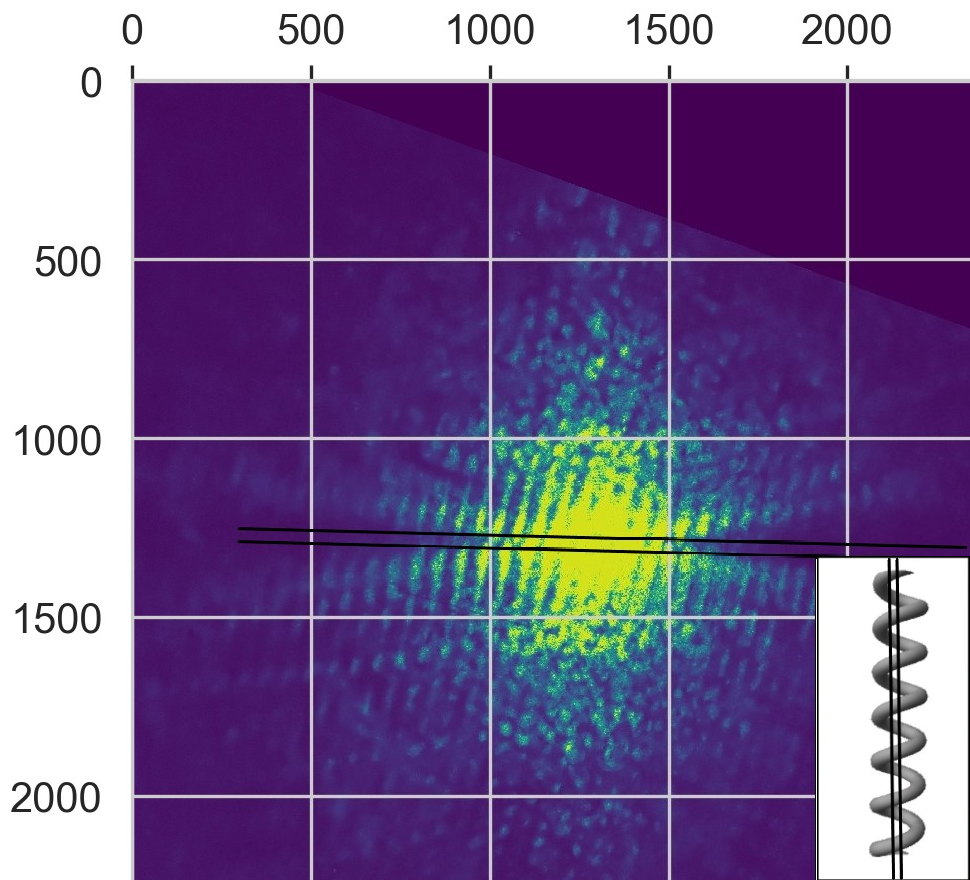
\includegraphics[width=\columnwidth]{figures/HelixSection1.png} % second figure itself
        \caption{N-slits section}
        \label{fig:HelixSection1}
    \end{subfigure}
    \begin{subfigure}{0.48\columnwidth}
        \centering
        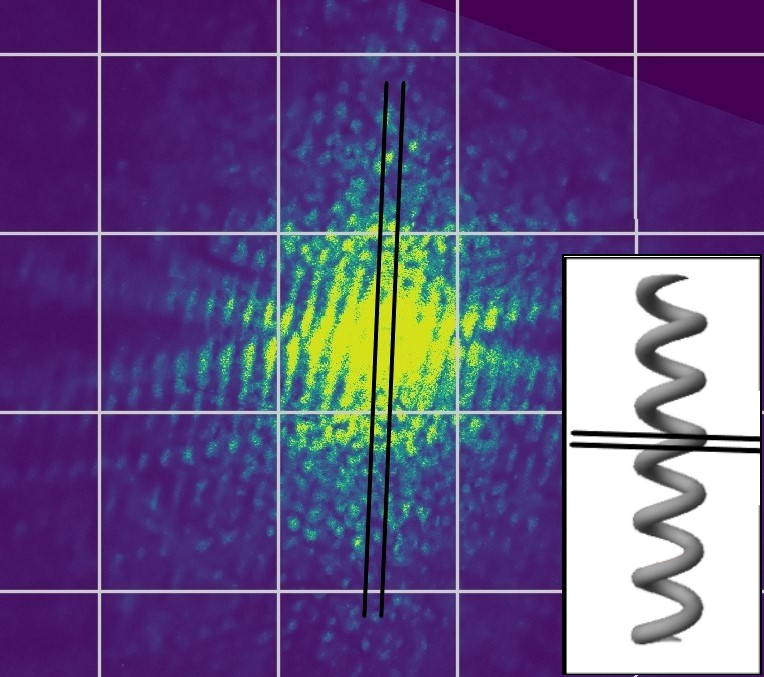
\includegraphics[width=\columnwidth]{figures/HelixSection2.png}
        \caption{Single slit section}
        \label{fig:HelixSection2}
    \end{subfigure}
    \begin{subfigure}{0.46\columnwidth}
        \centering
        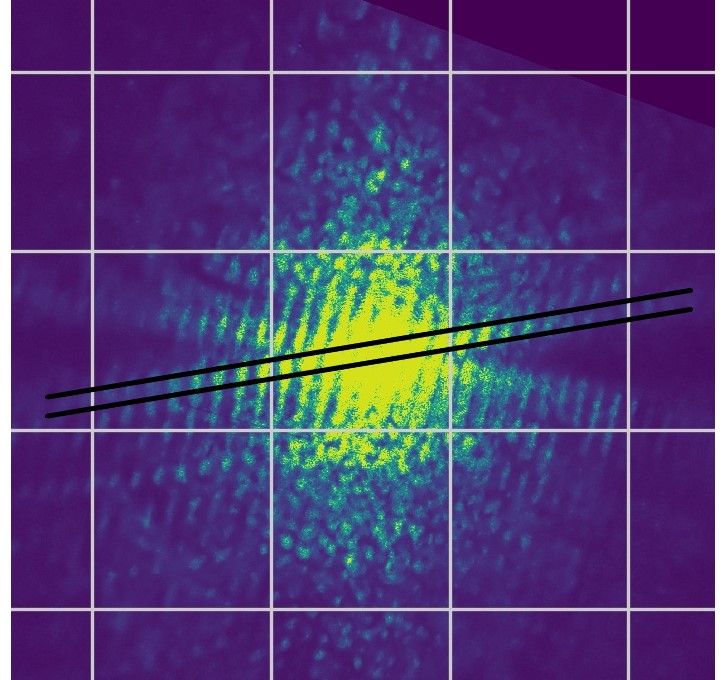
\includegraphics[width=\columnwidth]{figures/HelixSection4.jpg} % second figure itself
        \caption{"X" section 1}
        \label{fig:HelixSection3}
    \end{subfigure}
    \begin{subfigure}{0.48\columnwidth}
        \centering
        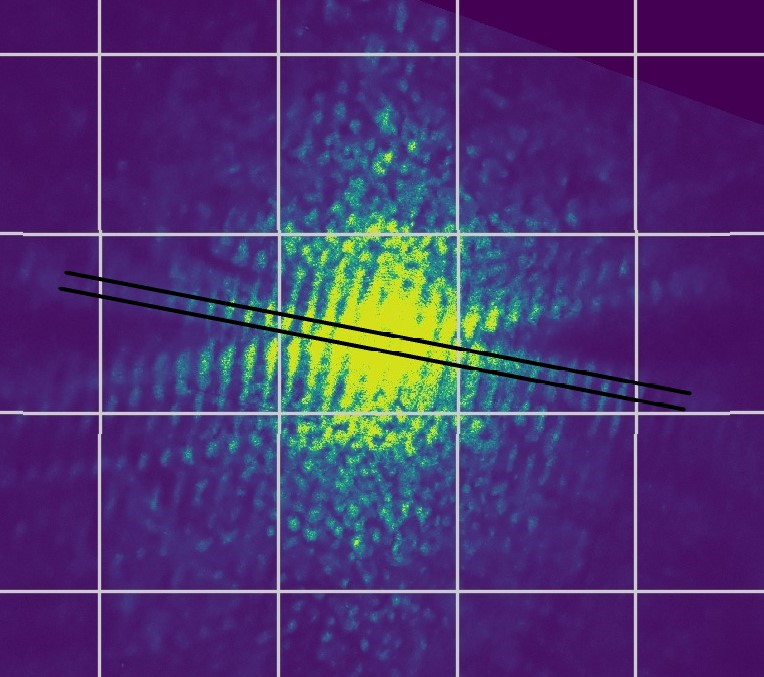
\includegraphics[width=\columnwidth]{figures/HelixSection3.jpg} % second figure itself
        \caption{"X" section 2}
        \label{fig:HelixSection4}
    \end{subfigure}
    \caption{Deconstruction of diffraction pattern to known 1D sections. The ticks shown are for pixels where $60[pixel]\approx 0.5[cm]$}
    \label{fig:HelixSections}
\end{figure}